\section{Aufgabe1}
\label{sec:Aufgabe1}
%\lstinputlisting[language=Python, firstline=15, lastline=21]{plots/plot.py}
Um $x$ Zufallszahlen mit der Rückweisungsmethode zu ziehen, müssen zwei mal $x$ Zahlen
gezogen werden, welche einem x-Wert und einem y-Wert zugeordnet werden.
Das Intervall für die x-Werte war mit $x=0$ und $x=20$ eingegrenzt. Die Untergrenze
der y-Werte liegt bei $0$ und für den maximal möglichen Wert wurde das Maximum der
Planck-Verteilung numerisch bestimmt. Die Rechung ist in \ref{fig:Rechnung} zu finden.\\
Die Ableitung wurde gebildet und mit \textbf{scipy.optimize.brentq} die Nullstelle bestimmt.\\
\begin{figure}
  \centering
  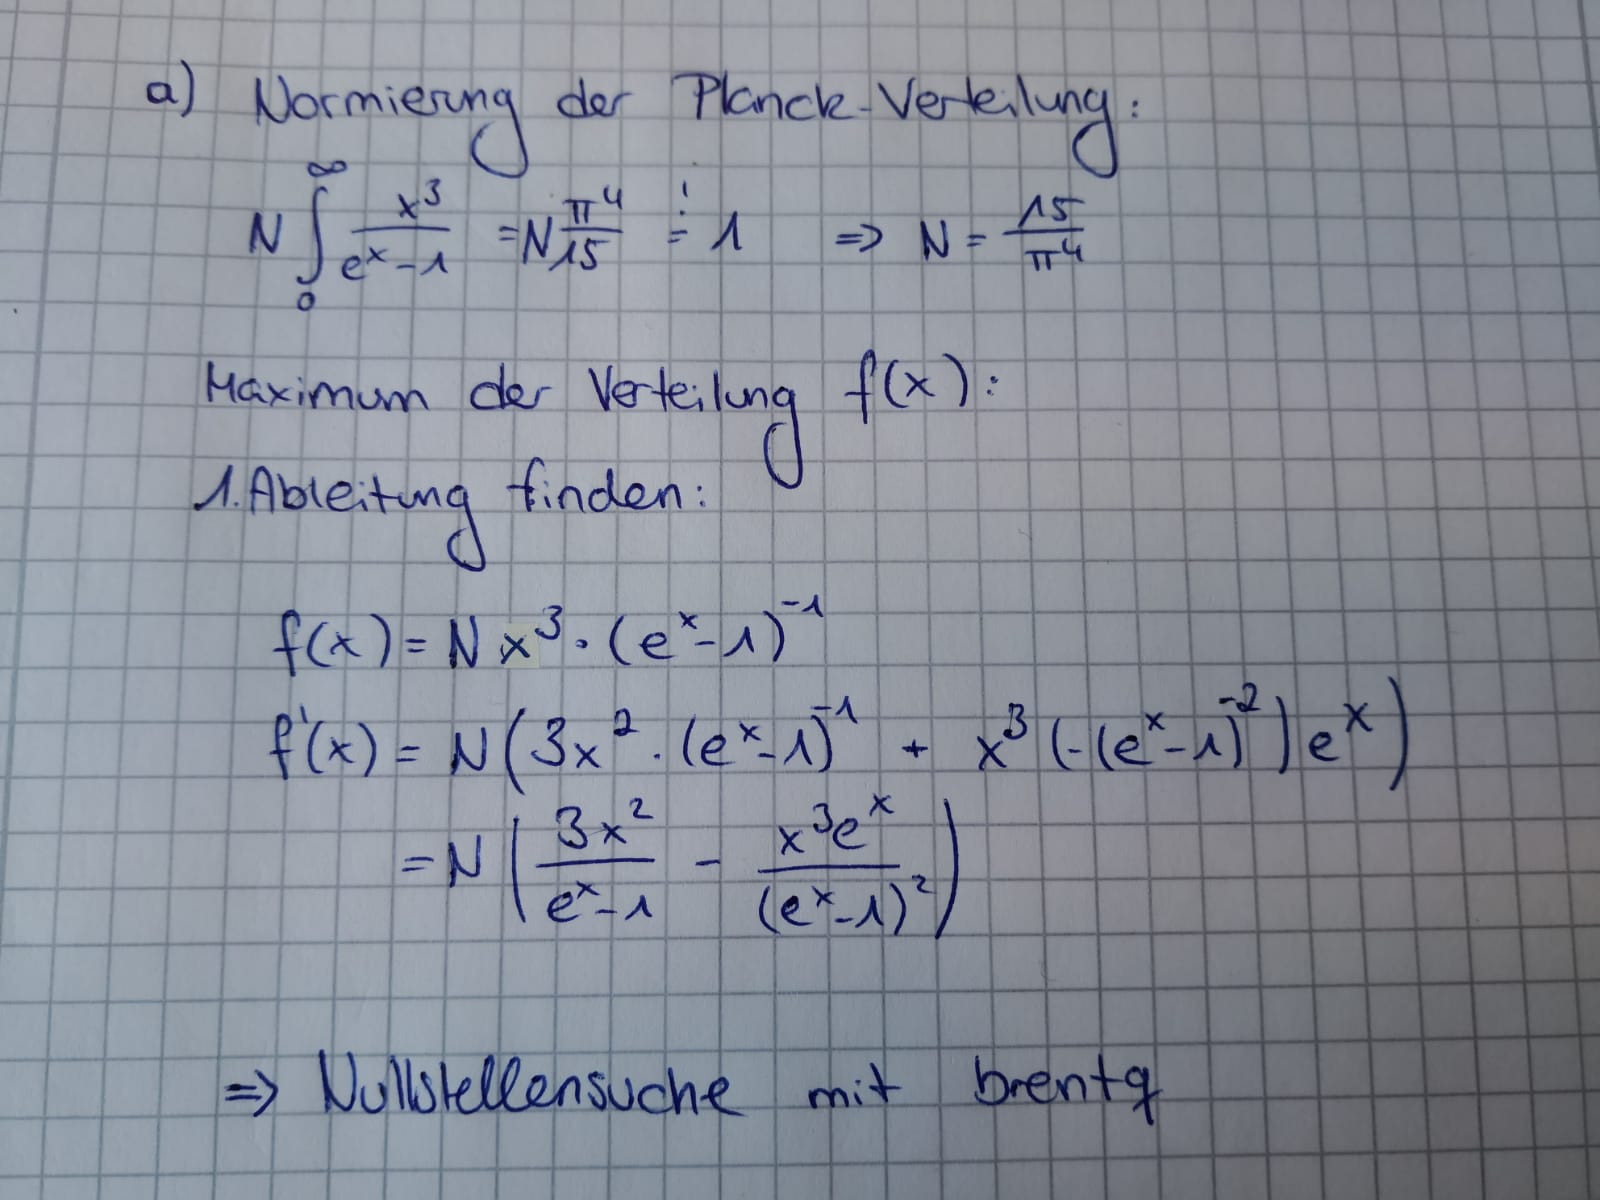
\includegraphics[height = 8cm]{pics/Rechnung1a.jpeg}
  \caption{Rechnung der Normierung und ersten Ableitung.}
  \label{fig:Rechnung}
\end{figure}
Als Grenze ergibt sich $y_{\text{max}} = 0.21888647009110665$. \\
Es werden nun immer zwei Zufallszahlen gezogen und als (x,y) Punkt interpretiert.
Gilt nun
\begin{equation*}
  y_{\text{zufall}}\leq f(x_{\text{zufall}})
\end{equation*}
wird das Zufallspaar akzeptiert und gespeichert, sonst verworfen. Eine while-Schleife
durchläuft dieses Verfahren bis $10^5$ Paare gefunden worden sind. Die x-Werte entsprechen den
gesuchten Zufallszahlen und sind in \ref{fig:Histogrammundso} aufgetragen.
\begin{figure}
  \centering
  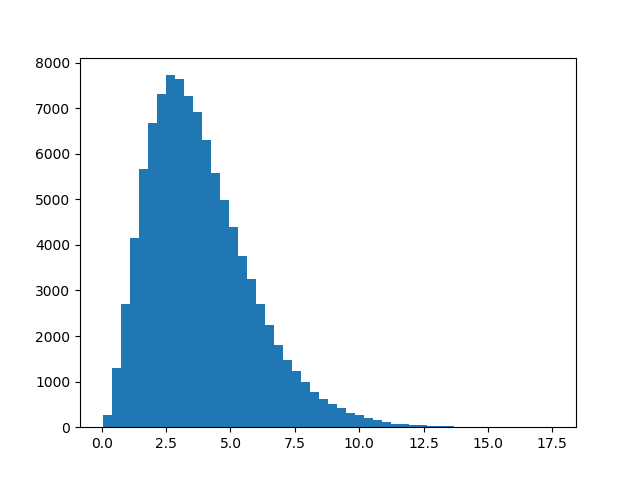
\includegraphics[height = 10cm]{plots/Histogramm.png}
  \caption{Zufallszahlen nach der Planck Verteilung.}
  \label{fig:Rechnung}
\end{figure}
Dabei wurden $339253$ Zufallszahlen verworfen und die Methode hat im Durchschnitt
$3,3$ Sekunden gebraucht.\\
Um die Zahl der verworfenen Zahlen zu minimieren wird eine gestückelte Majorante
$g(x)$ definiert. Diese ist in \ref{fig:Mayo} dagestellt.
\begin{figure}
  \centering
  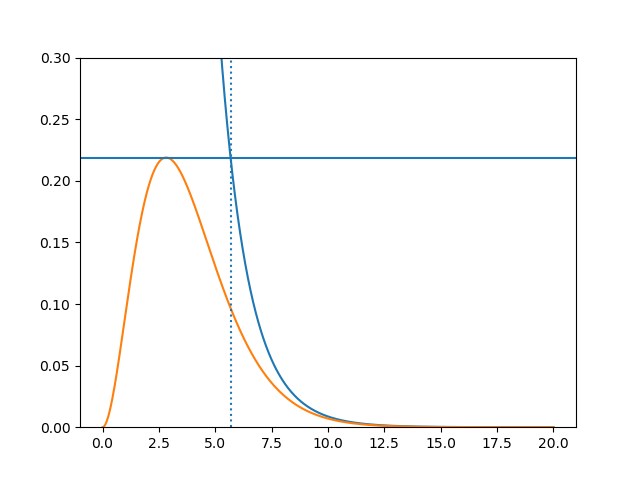
\includegraphics[height = 10cm]{plots/Majoranten.png}
  \caption{Planckverteilung und die Majoranten.}
  \label{fig:Mayo}
\end{figure}
Es kann eine Transformationsmethode
verwendet werden, weil die Stammfunktion von $g(x)$ intervierbar ist
und dies für die Methode benötigt wird.
Um ein Samplen aus dieser Verteilung zu ermöglichen muss die Funktion normiert werden.
Die Rechnung ist in \ref{fig:Rech} zu finden.
\begin{figure}
  \centering
  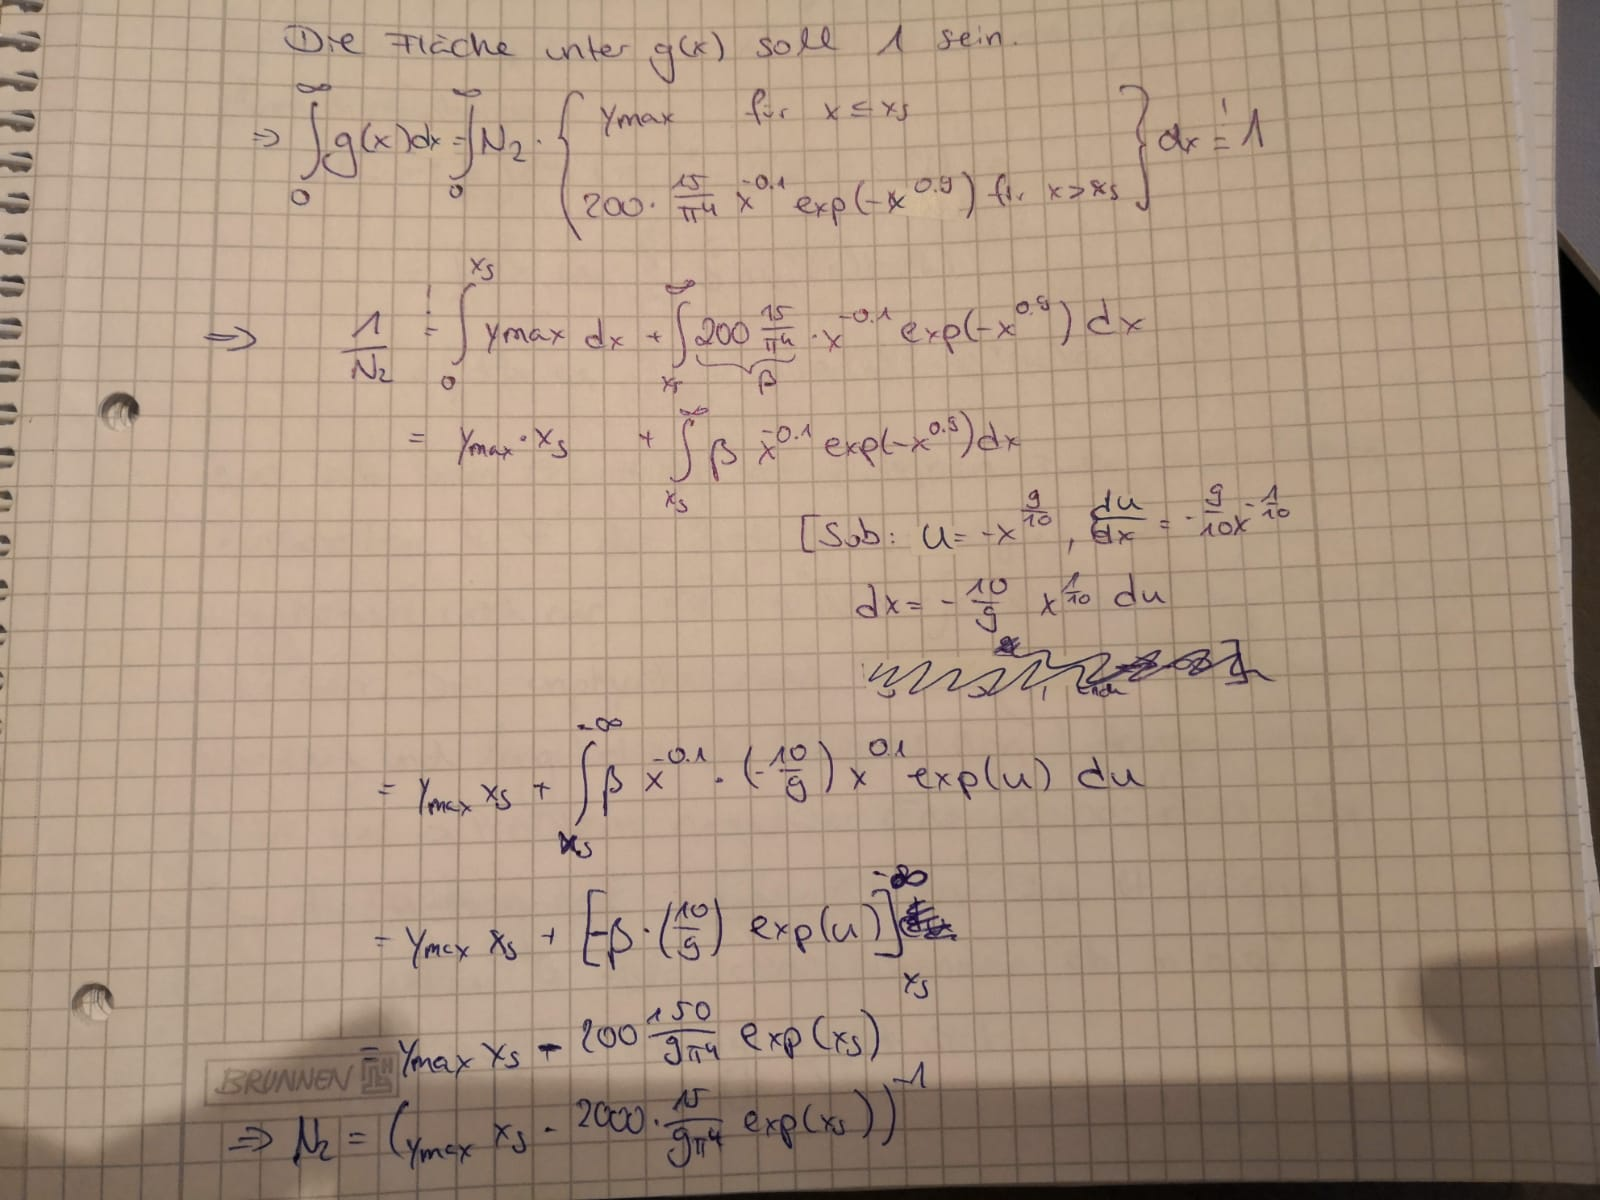
\includegraphics[height = 10cm]{pics/Rechnung2b.jpeg}
  \caption{Berechnung der Normierung für g(x)}
  \label{fig:Rech}
\end{figure}
